\begin{frame}[fragile]{Tutorial: Two-site fidelity optimization}

\begin{columns}

\begin{column}{5cm}

\begin{onlyenv}<1->
\begin{lstlisting}[language=JuliaLocal, style=julia, mathescape, basicstyle=\small]
$\psi_0$ = Zp1 * Zp2
$\psi$ = (ZpZp + ZmZm) / √2



function F($\theta$)
  $\psi_\theta$ = apply(U($\theta$, i1, i2), $\psi_0$)
  return -abs(inner($\psi$, $\psi_\theta$))^2
end
\end{lstlisting}
\end{onlyenv}

\begin{onlyenv}<3->
\begin{lstlisting}[language=JuliaLocal, style=julia, mathescape, basicstyle=\small]
$\theta_0$ = [0, 0, 0, 0]
$\theta$ = minimize(F, $\partial$F, $\theta_0$;
        nsteps=50, $\gamma$=0.1)

F($\theta_0$), norm($\partial$F($\theta_0$))
F($\theta$), norm($\partial$F($\theta$))
 \end{lstlisting}

\end{onlyenv}
\end{column}

\begin{column}{5cm}

\begin{onlyenv}<1-1>
Reference state: \\
|0$\rangle$ = |Z+Z+$\rangle$ \\
~\\
Target state: \\
|$\psi\rangle$ = (|Z+Z+$\rangle$ + \\
          |Z-Z-$\rangle$)/√2 \\
~\\
Find $\theta$ that minimizes: \\
F($\theta$) = -|$\langle\psi$|U($\theta$)|0$\rangle$|$^2$
\end{onlyenv}

\begin{onlyenv}<2->
\vspace*{0.0cm}
\begin{center}
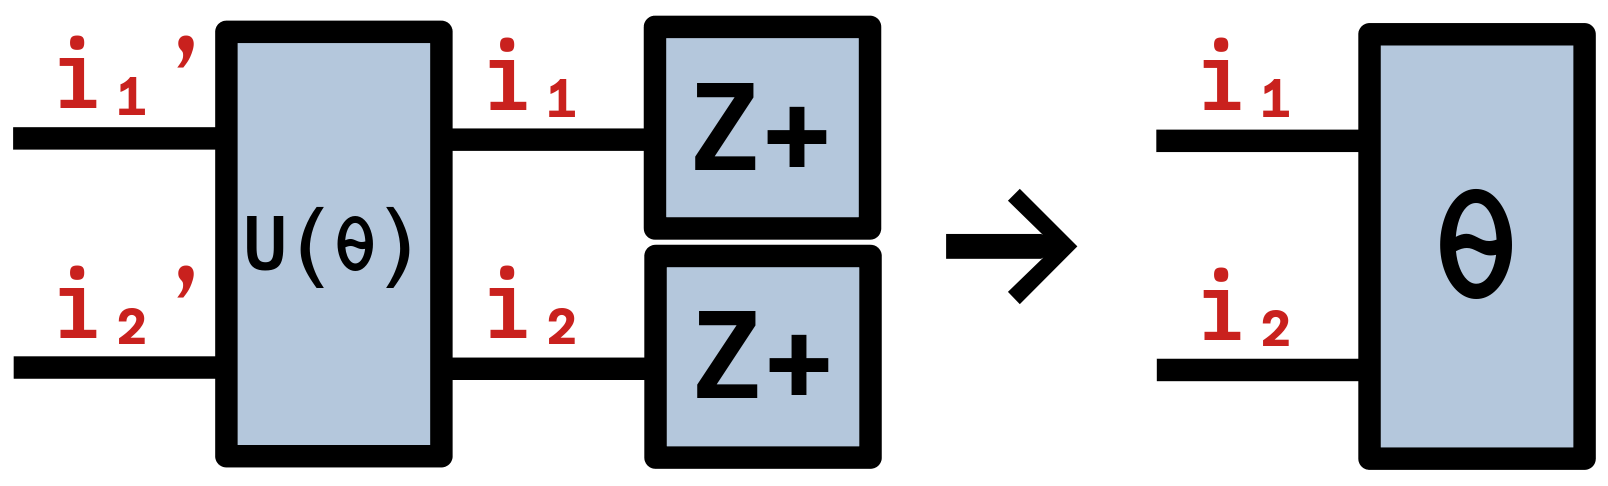
\includegraphics[width=0.2\textwidth]{
  slides/assets/UZp1Zp2.png
} \\
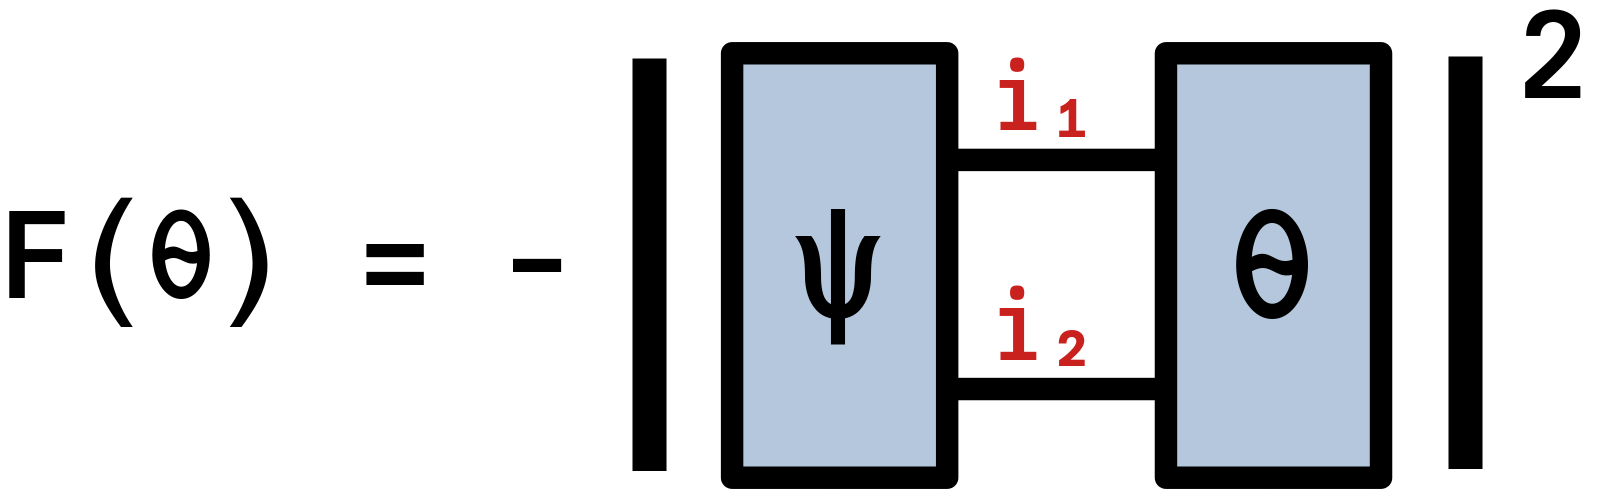
\includegraphics[width=0.2\textwidth]{
  slides/assets/psi12theta12.png
}
\end{center}
\vspace*{0.0cm}
\end{onlyenv}

\begin{onlyenv}<3-3>
~\\
~\\
~\\
~\\
$\approx$ (-0.5, 0.5) \\
$\approx$ (-0.9938992, 0.07786879) \\
    $\approx$ (-1, 0)
\end{onlyenv}

\begin{onlyenv}<4->
\vspace*{0.0cm}
\begin{center}
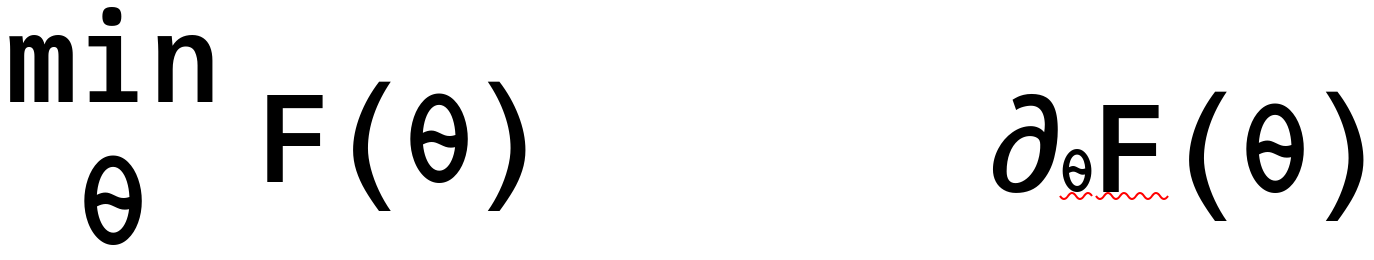
\includegraphics[width=0.2\textwidth]{
  slides/assets/min_grad_F_theta.png
}
\end{center}
\vspace*{0.0cm}
\end{onlyenv}

\end{column}

\end{columns}

\end{frame}
